\section{推理循环与软件栈}

LeRobot 的在线推理是一个持续运行的帧循环。
从系统行为看，每一帧可以划分为观测、推理、执行和等待四个阶段：
观测阶段收集相机图像与机械臂关节状态，推理阶段根据当前观测计算下一步动作，
执行阶段将动作写入舵机，等待阶段则用于补足目标帧率所需的帧间隔。
四个阶段在单个 Python 进程内串行推进，不依赖外部消息中间件；
若以 30\,fps 作为控制目标，则单帧可用时间约为 33.3\,ms。

\begin{figure}[htbp]
  \centering
  \begingroup
\definecolor{recordFrame}{HTML}{E5E7EB}
\definecolor{recordStageFill}{HTML}{F8FBFF}
\definecolor{recordBlue}{HTML}{2563EB}
\definecolor{recordWaitFill}{HTML}{FFFAF2}
\definecolor{recordOrange}{HTML}{F97316}
\definecolor{recordAsyncFill}{HTML}{F9FAFB}
\definecolor{recordGray}{HTML}{6B7280}
\definecolor{recordText}{HTML}{111827}
\definecolor{recordSubText}{HTML}{4B5563}
\definecolor{recordSmallText}{HTML}{374151}
\resizebox{\textwidth}{!}{%
\begin{tikzpicture}[
  x=1pt,
  y=-1pt,
  >=Triangle,
  stage/.style={
    rounded corners=10pt,
    draw=recordBlue,
    line width=2.4pt,
    fill=recordStageFill,
  },
  wait/.style={
    rounded corners=10pt,
    draw=recordOrange,
    line width=2.4pt,
    fill=recordWaitFill,
  },
  async/.style={
    rounded corners=9pt,
    draw=recordGray,
    line width=1.8pt,
    dashed,
    dash pattern=on 7pt off 5pt,
    fill=recordAsyncFill,
  },
  flow/.style={
    draw=recordBlue,
    line width=3.2pt,
    -{Triangle[length=18pt,width=21pt]},
  },
  loop/.style={
    draw=recordGray,
    line width=2.8pt,
    rounded corners=0pt,
    -{Triangle[length=18pt,width=21pt]},
  },
  asyncFlow/.style={
    draw=recordGray,
    line width=2.2pt,
    dashed,
    dash pattern=on 7pt off 5pt,
    -{Triangle[length=18pt,width=21pt]},
  },
]
  \path[use as bounding box] (0,0) rectangle (1080,360);

  \draw[rounded corners=18pt, draw=recordFrame, line width=1.5pt, fill=white]
    (28,28) rectangle (1052,332);

  \draw[stage] (104,88) rectangle (294,184);
  \node[font=\bfseries\fontsize{34}{40}\selectfont, text=recordText] at (199,128) {观测阶段};
  \node[font=\fontsize{24}{30}\selectfont, text=recordSubText] at (199,164) {Observation};

  \draw[stage] (332,88) rectangle (522,184);
  \node[font=\bfseries\fontsize{34}{40}\selectfont, text=recordText] at (427,128) {推理阶段};
  \node[font=\fontsize{24}{30}\selectfont, text=recordSubText] at (427,164) {Inference};

  \draw[stage] (560,88) rectangle (750,184);
  \node[font=\bfseries\fontsize{34}{40}\selectfont, text=recordText] at (655,128) {执行阶段};
  \node[font=\fontsize{24}{30}\selectfont, text=recordSubText] at (655,164) {Execution};

  \draw[wait] (788,88) rectangle (978,184);
  \node[font=\bfseries\fontsize{34}{40}\selectfont, text=recordText] at (883,128) {等待阶段};
  \node[font=\fontsize{24}{30}\selectfont, text=recordSubText] at (883,164) {Wait};

  \draw[flow] (294,136) -- (332,136);
  \draw[flow] (522,136) -- (560,136);
  \draw[flow] (750,136) -- (788,136);

  \draw[loop] (883,88) -- (883,58) -- (199,58) -- (199,88);
  \node[
    font=\fontsize{18}{23}\selectfont,
    text=recordSubText,
    fill=white,
    inner xsep=22pt,
    inner ysep=2pt,
  ] at (540,57) {等待结束后进入下一帧};

  \draw[async] (74,230) rectangle (324,294);
  \node[font=\bfseries\fontsize{22}{28}\selectfont, text=recordSmallText] at (199,256) {异步读摄像头线程};
  \node[font=\fontsize{18}{24}\selectfont, text=recordGray] at (199,281) {Camera Prefetch Thread};

  \draw[asyncFlow] (199,184) -- (199,230);
\end{tikzpicture}%
}
\endgroup

  \caption{LeRobot 单帧推理循环流程}
  \label{fig:record-loop}
\end{figure}

图~\ref{fig:record-loop} 只保留在线控制循环的阶段边界：
主线程按观测、推理、执行和等待的顺序推进一帧，等待结束后进入下一帧。
摄像头图像并不是每一帧都由主线程直接阻塞读取，而是由后台线程持续预取，
观测阶段再从该线程维护的缓存中取回最近可用的图像帧。

为说明推理循环背后的调用边界，本文将在线推理软件栈归纳为四层架构：
应用逻辑层、库与驱动层、glibc 运行时层以及 Linux 内核层（图~\ref{fig:lerobot-stack}）。
每个阶段沿不同的软件栈路径向下调用：
观测阶段同时采集摄像头图像和关节角度——
摄像头图像通过 OpenCV 后台线程异步预取，主线程取回已解码缓存帧，
底层经由 V4L2 驱动和内核 pselect6 等待帧就绪；
关节角度由 scservo\_sdk 通过 pyserial 向舵机总线发起同步读取，
底层经由串口驱动和内核 read/write 系统调用完成半双工通信。
推理阶段将观测张量送入 ACT 策略网络，
由 PyTorch（C10 线程池 + ARM NEON 算子）在 CPU 上完成前向计算，
经由 glibc 和 Linux 内核的 futex 机制协调线程同步。
执行阶段将预测动作通过 scservo\_sdk 写回舵机，
路径与观测阶段的关节读取对称。等待阶段由 busy\_wait 函数补足帧间隔；
在树莓派 Linux 环境下，该函数会调用 time.sleep，
底层通常通过 clock\_nanosleep 进入内核定时睡眠路径，使进程主动让出 CPU。

\begin{figure}[H]
  \centering
  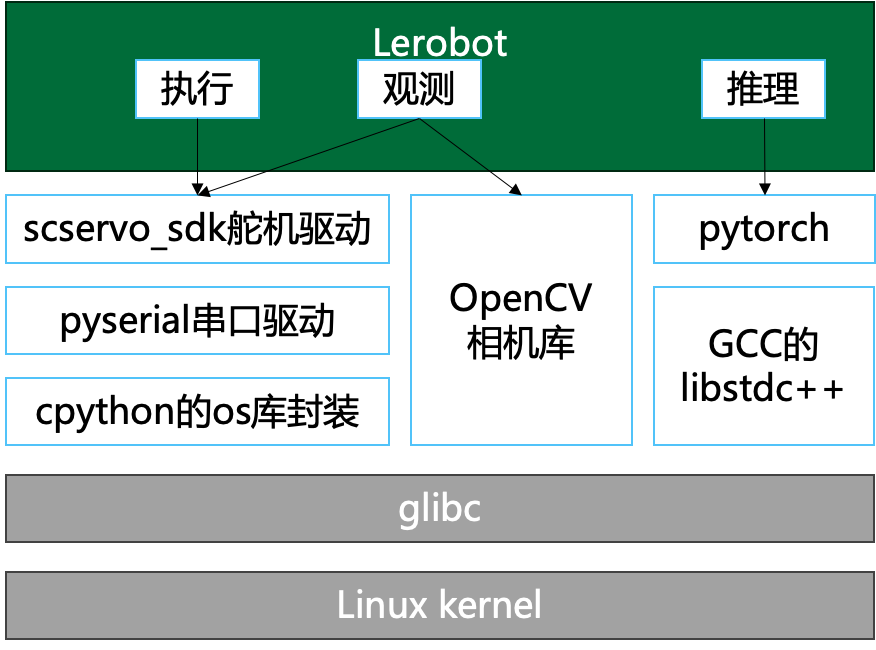
\includegraphics[width=0.9\textwidth]{2_实验环境构建/image/lerobot_stack.png}
  \caption{Lerobot软件栈架构}
  \label{fig:lerobot-stack}
\end{figure}

图~\ref{fig:lerobot-stack} 从上到下展示了 LeRobot 在线推理经过的四个软件层次。
最上层是由在线控制程序组织的应用逻辑，它按照观测、推理、执行和等待的顺序推进每一帧；
中间的库与驱动层承担具体工作，例如 OpenCV 负责图像读取，PyTorch 负责神经网络前向计算，
scservo\_sdk 与 pyserial 负责舵机总线通信；
再向下，glibc 将线程同步、休眠、读写等运行时操作转化为系统调用；
最底层的 Linux 内核则实际调度 CPU、管理摄像头和串口设备，并把数据传递给硬件。
因此，这张图说明的是：一次推理循环虽然写在 Python 代码中，
但它的执行过程会逐层穿过第三方库、运行时和内核，最终落到 ARM CPU 与外设驱动上。
